Suppose $N\ge 1$ is an integer and define $h = 1/(N + 1)$ and $x_j = jh$ for $j = 0,\ldots,N + 1$. Consider the $N+2$ hat functions, defined for $x\in[0,1]$ as
\[
\phi_k(x) = \left\{\begin{array}{ll}
(x-x_{k-1})/h, & x\in[x_{k-1},x_k);\\
(x_{k+1}-x)/h, & x\in[x_k,x_{k+1});\\
0,& \mbox{otherwise;}
\end{array}\right.
\]
for $k=1,\ldots, N$, with
\[
\phi_0(x) = \left\{\begin{array}{ll}
(x_1-x)/h, & x\in[x_0,x_1);\\
0,& \mbox{otherwise;}
\end{array}\right.
\]
and
\[
\phi_{N+1}(x) = \left\{\begin{array}{ll}
(x-x_N)/h, & x\in[x_N,x_{N+1}];\\
0,& \mbox{otherwise.}
\end{array}\right.
\]
We call these piecewise linear functions {\em hat functions} 
because of their shape.  They will be important functions later in the course.  
For example, when $N=9$ and $k=3$, this function takes the following form.
\begin{center}
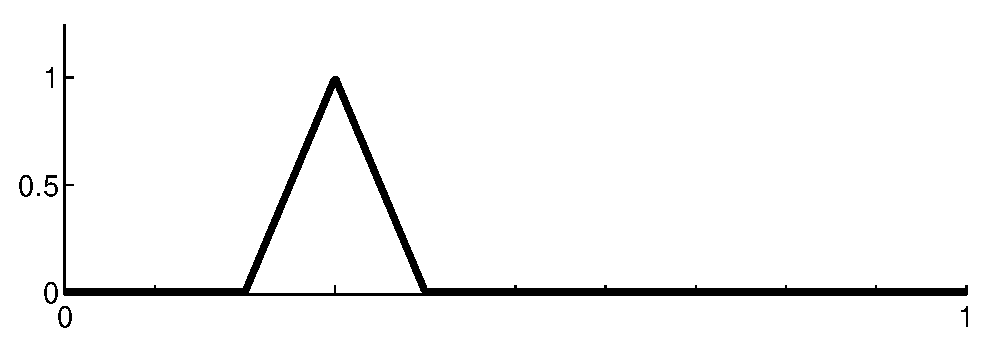
\includegraphics[scale=0.6]{plothat}
\begin{picture}(0,0)
\put(-215,0){$x_2$}
\put(-190,0){$x_3$}
\put(-165,0){$x_4$}
\put(-175,50){$\phi_3(x)$}
\end{picture}
\end{center}

\begin{enumerate}
\item Write a MATLAB function for $\phi_k(x)$.  It should take in as input $x$, $k$, and $N$.  It should return the value $\phi_k(x)$.  It should also be able to take in a vector for $\Bx=(\hat{x}_1,\ldots,\hat{x}_m)$ and return the vector $\phi_k(\Bx)=(\phi_k(\hat{x}_1),\ldots,\phi_k(\hat{x}_m))$.
\\
\item Let $N=9$.  Plot $\phi_0(x),\phi_4(x), \phi_5(x),\phi_6(x), \phi_{10}(x)$ on the same figure.  Make sure to:
\begin{itemize}
\item plot each function with a different color;
\item label the axes and provide a title;
\item create an accurate legend for the figure;
\item adjust the text sizes if necessary to make everything easily legible;
\item use the LATEX interpreter to make your labels, titles, and legend look stylish.
\end{itemize}
\end{enumerate}

%%%%%%%%%%%%%%%%%%%%%%%%%%%%%%%%%%%%%%%%%%%%%%%%%%%%%%%%%%%%%%%%%%%%%%%%%%%%%%%%
\ifthenelse{\boolean{showsols}}{\input codeHat_sol}{}

